\documentclass[
%a4paper,12pt
encoding=utf8
]{../twoeskd}

% Packages required by doxygen
\usepackage{fixltx2e}
\usepackage{calc}
\usepackage{doxygen}
\usepackage[export]{adjustbox} % also loads graphicx
\usepackage{graphicx}
\usepackage[utf8]{inputenc}
\usepackage{makeidx}
\usepackage{multicol}
\usepackage{multirow}
\PassOptionsToPackage{warn}{textcomp}
\usepackage{textcomp}
\usepackage[nointegrals]{wasysym}

% NLS support packages
\usepackage[T2A]{fontenc}
\usepackage[russian]{babel}

% Font selection
\usepackage{courier}
\usepackage{amssymb}
\usepackage{sectsty}
\renewcommand{\familydefault}{\sfdefault}
\newcommand{\+}{\discretionary{\mbox{\scriptsize$\hookleftarrow$}}{}{}}

% Page & text layout
\usepackage{geometry}
\tolerance=750
\hfuzz=15pt
\hbadness=750
\setlength{\emergencystretch}{15pt}
\setlength{\parindent}{0cm}
\setlength{\parskip}{0.2cm}
\makeatletter
\makeatother

% Headers & footers
% \usepackage{fancyhdr}
% \renewcommand{\sectionmark}[1]{%
%   \markright{\thesection\ #1}%
% }

% Indices & bibliography
\usepackage{natbib}
\usepackage[titles]{tocloft}
\setcounter{tocdepth}{3}
\setcounter{secnumdepth}{5}
\makeindex

% Custom commands
\newcommand{\clearemptydoublepage}{%
  \newpage{\pagestyle{empty}\cleardoublepage}%
}
\renewcommand{\DoxyLabelFont}{%
  \fontseries{bc}\selectfont%
}

% Custom packages
\usepackage{pdfpages}


\setlength{\parindent}{0cm}
\setlength{\parskip}{0.2cm}

\usepackage{listings}

% debug to see the frame borders
% from https://en.wikibooks.org/wiki/LaTeX/Page_Layout
% \usepackage{showframe}

% change style of titles in \section{}
\usepackage{titlesec}
\titleformat{\section}[hang]{\huge\bfseries\center}{\thetitle.}{1em}{}
\titleformat{\subsection}[hang]{\Large\raggedright}{\thetitle.}{1em}{\underline}
\titleformat{\subsubsection}[hang]{\large\raggedright}{\thetitle.}{1pt}{}
\titleformat{\paragraph}[hang]{\large\raggedright}{\thetitle.}{0.3pt}{}

% Packages for text layout in normal mode
% \usepackage[parfill]{parskip} % автоматом делает пустые линии между параграфами, там где они есть в тексте
% \usepackage{indentfirst} % indent even in first paragraph
\usepackage{setspace}	 % controls space between lines
\setstretch{1} % space between lines
\setlength\parindent{0.9cm} % size of indent for every paragraph
\usepackage{csquotes}% превратить " " в красивые двойные кавычки
\MakeOuterQuote{"}


% this makes items spacing single-spaced in enumerations.
\newenvironment{my_enumerate}{
\begin{enumerate}
  \setlength{\itemsep}{1pt}
  \setlength{\parskip}{0pt}
  \setlength{\parsep}{0pt}}{\end{enumerate}
}


% Custom commands
% configure eskd
\titleTop{
\textbf{\Large ПРАВИТЕЛЬСТВО РОССИЙСКОЙ ФЕДЕРАЦИИ \\
НАЦИОНАЛЬНЫЙ ИССЛЕДОВАТЕЛЬСКИЙ УНИВЕРСИТЕТ \\
«ВЫСШАЯ ШКОЛА ЭКОНОМИКИ» } \\
\vspace*{0.2cm}
{\small Факультет компьютерных наук \\
Департамент программнoй инженерии \\
}
}
\titleDesignedBy{Студент группы БПИ 151 НИУ ВШЭ}{Абрамов А.M.}
\titleAgreedBy{%
\parbox[t]{7cm} {
Доцент департамента \\
программной инженерии \\
факультета компьютерных наук \\
канд. техн. наук \\
}}{Р. З. Ахметсафина}
\titleApprovedBy{
\parbox[t]{10cm} {
Академический руководитель \\
образовательной программы \\
«Программная инженерия» \\
профессор департамента программной \\
инженерии канд. техн. наук \\
}}{В. В. Шилов}
\titleName{ПРОГРАММА СКЕЛЕТНАЯ АНИМАЦИЯ}
\workTypeId{RU.17701729.509000 T3 01-1-ЛУ}

\titleSubname{Пояснительная записка}


%===== C O N T E N T S =====
\begin{document}

% Titlepage & ToC
\pagenumbering{roman}

% some water filling text, that is pointless but adds text
% \newpage

\begin{center}
{\large АННОТАЦИЯ}
\end{center}

Настоящий документ представляет собой техническое задание для разработки приложения реализации алгоритма скелетной анимации. Данный документ составлен в соответствии с ГОСТ. В документе содержатся следующие разделы: «Введение», «Основания для разработки», «Назначение разработки», «Требования к программе», «Технико-экономические характеристики», «Стадии и этапы разработки», «Порядок контроля и приемки».

В разделе «Введение» содержится информация о намиеновании и краткой характеристике разрабатываемого приложения.

В разделе «Основания для разработки» содержится информация о документах, на основании которых ведется разработка настоящего приложения, а так же наименование темы разработки.

В разделе «Назначение разработки» содержится информация о функциональном и эксплуатационном назначении разрабатываемого прилоежния.

В разделе «Требования к программному изделию» содержится информация о требованиях к функциональным характеристикам, требованиях к надежности, условиях эксплуатации, требованиях к составу и параметрам технических средств, требования к информационной и программной совместимости.

В разделе «Требования к программной документации» содержится информация о требованиях, в соответствии с которыми должна выполняться разработка программной документации приложения.

В разделе «Технико-экономические показатели» содержится информация об ориентировочной экономической эффективности и ожидаемой годовой потребности, экономических преимуществах разработки по сравнению с лучшими зарубежными и отечественными аналогами.

В разделе «Стадии и этапы разработки» содержится информация о необходимых стадиях разработки, этапах и содержании работ. Присутствует информация о сроках разработки и исполнителях.

В разделе «Порядок контроля и приемки» содержится подробная информация о видах испытаний, которые будут применены к данному приложению, а так же общих требованиях к приемке работ.

Перед прочтением настоящего документа рекомендуется ознакомиться со списком терминов, для предотвращения непонятных моментов.



\newpage
\pagenumbering{arabic}
\tableofcontents
% \pagenumbering{arabic}

% --- add my custom headers ---
\newpage
\section{Введение}
\subsection{Наименование}
Наименование: «Программа скелетная анимация». Англ.: «Program of Skeletal Animation».


\subsection{Краткая характеристика}
    Цель работы - реализовать систему скелетной анимации. 
    В основные задачи работы входит загрузка анимации из этих файлов, рассчет промежуточных кадров анимации и воспроизведение анимации на экране средствами OpenGL. 
    Также программа предоставляет пользовтелю возможность рассмотреть анимацию с разных ракурсов, перейти к любому моменту времени в анимации и просмотреть иерархию костей и модели.
В состав работы также входит создание демонстрационных исходных данных (файлов) для данной системы.



\newpage
\section{Назначение разработки}
\subsection{Функциональное значение}
Функциональным назначением приложения является предоставление пользователю возможности быстро загрузить несколько анимаций из файла или нескольких файлов, просмотреть из, просмотреть информацию об отдельных составляющих каждой анимации, проиграть ее с разной скоростью и в произвольном напралении, проверить каждую анимацию на правильность формата.

\subsection{Эскплутационное значение}
Программа наглядно демонстрирует содержание файла экпортированного из пакетов для 3-х мерного моделированния. Она должна использоваться в процессе отладки приложений использующих анимацию и в работе дизайнера  3D моделей.


\newpage
\section{Технические характеристики}
\subsection{Постановка задачи на разработку программы}
    Цель работы - реализовать программу скелетной анимации.

\bigskip
Задачи работы:

\smallskip
\begin{my_enumerate}
\item Создание исходных данных (файлов) для скелетной анимации.
\item Загрузка анимации из файла (содержание описанно в ТЗ).
\item Рассчет кадров анимации.
\item Воспроизведение анимации на экране средствами OpenGL.
\item Предоставление пользователю возможности перейти к любому моменту времени в анимации.
\item Отрисовка костей модели.
\item Возможность вкл./выкл. учет нормалей и материалов во время отрисовки.
\item Поддержка двух видов камер в OpenGL. Первый вид это камера, движение которой сковано орбитой вокруг модели, и другой тип это камера двигающаяся совершенно свободно.
\end{my_enumerate}


\subsection{Описание алгоритма и функционирования программы}


%=============================================================
\subsubsection{Выбор алгоритма}

\paragraph{Различные подходы}
к созданию программ трех мерной анимации балансируют между методами с большим количеством вычислений и методами, требующими большого объема памяти. Условно можно выделить явные и неявные системы анимации.

\paragraph{Явные системы анимации} хранят отдельную модель для каждого кадра.
После записи данных в файл, существует много методов для воспроизведения анимации.
Такие методы требуют лишь элементарной математики.
Однако типичная запись одного трека анимации для одного персонажа занимает около 10MB (в формате MD3).

\begin{figure}[h!]
    \centering
    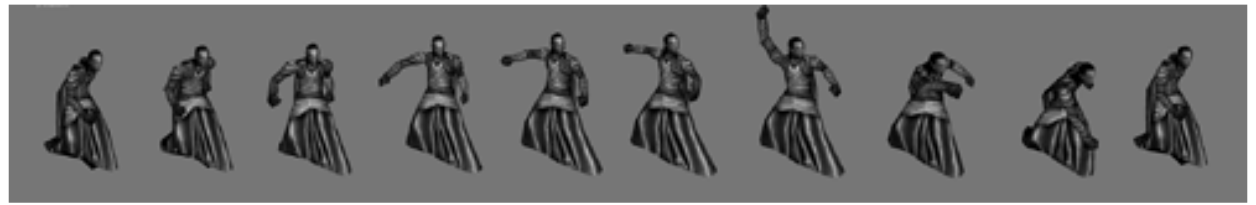
\includegraphics[width=0.8\textwidth]{explicit_animation.png}
    \caption{Каждому кадру соответствует своя модель}
\end{figure}

Предпочтение явным системам отдается, когда необходимо анимировать большие группы людей или животных.

\paragraph{Неявные системы анимации} хранят не модели, а более высокоуровневое описание движения.
В частности неявные \textbf{системы скелетной анимации} содержат описание (через матрицу поворота) для каждой кости, как например локоть, плечо, шея.
В реальном времени эти описания применяются к неанимированной модели для расчета следующего кадра анимации.
Эти расчеты обычно требуют сложной математики с матрицами и тригонометрией.
А следовательно и много CPU времени.


\begin{figure}[h!]
    \centering
    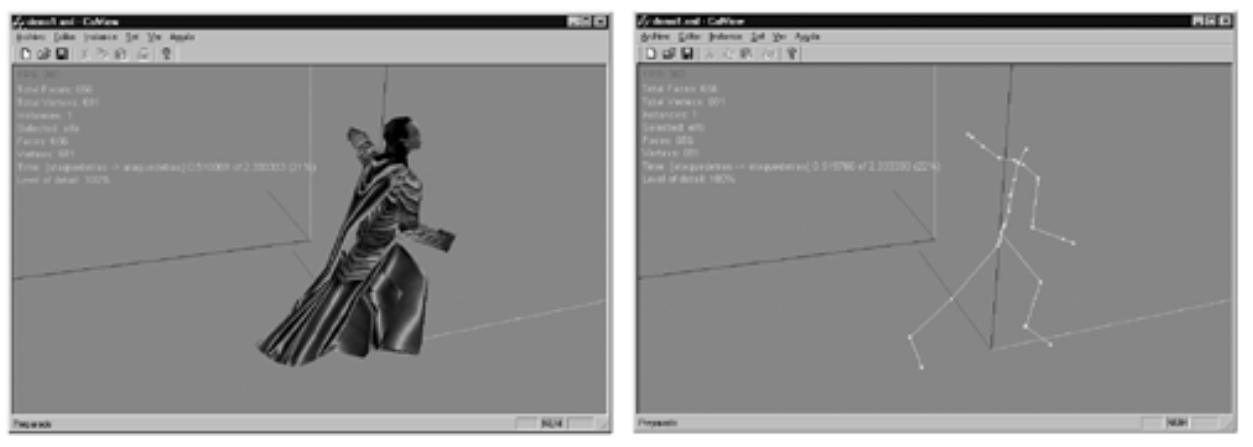
\includegraphics[width=0.8\textwidth]{implicit_animation.png}
    \caption{\small{Слева: анимированный персонаж; справа: скелет для данного кадра}}
    %\label{fig:awesome_image}
\end{figure}

Неявные системы используются, когда персонаж может совершать несколько действий одновременно и невозможно предугадать все возможные варианты анимации.

%=============================================================
\subsubsection{Основные определения и структуры данных}

\paragraph{Кость}
Каждая кость содержит информацию о трех мерной трансформации (которая состоит из поворота, растяжения и смещения), а также информацию о кости-отце. Глобальная трансформация кости-потомка, - это произведение глобальной трансформации кости-родителя на локальную трансформацию самой кости-потомка. Изменение транформации родителя, меняет трансформацию потомка.

Ниже приведен класс описывающий кость скелета:
\begin{small}
\begin{verbatim}
class BoneNode
{
    public string Name;
    public Matrix4 GlobalTransform;
    public Matrix4 LocalTransform;

    public BoneNode Parent;
    public List<BoneNode> Children;
    public BoneNode(Node node_data) { ... }
}
\end{verbatim}
\end{small}

\paragraph{Скелет}
Скелетом называют иерархичную (дeревообразную) структуру сформированную костями. Скелет определяеться с помощью корневой кости в иерархии.


\paragraph{Трек анимации}
В треке содержатся матрицы поворота скелета в ключевые моменты времени.
В упрощенном виде трек можно представить в качестве  массива пар: 
$\lbrace$ время ключевого кадра, массив из матриц поворота для каждой кости $\rbrace$

\begin{figure}[h!]
    \centering
    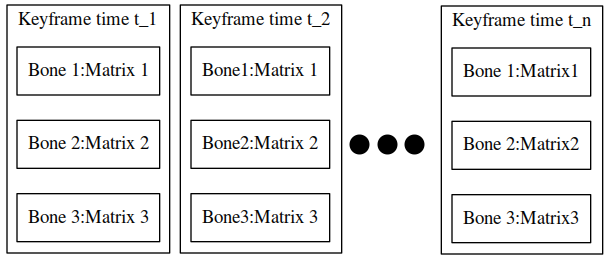
\includegraphics[width=0.4\textwidth]{anim_track.png}
    \caption{\small{В ключевые моменты времени \detokenize{(t_1, t_2, ... t_n)}, каждая кость ставиться в соответствие с матрицей локальной трансформации.}}
    
\end{figure}


\paragraph{Модель}
Модель состоит из набора вершин, весов вершин, нормалей, материалов. В пакете для трех мерной анимации модель привязывают к скелету, каждая вершина модели «привязывается» к какой-либо кости скелета (или к нескольким костям). После привязки модели к скелету при движении отдельной кости будут двигаются и все вершины, привязанные к ней.

\begin{figure}[h!]
    \centering
    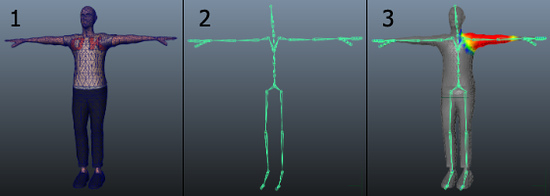
\includegraphics[width=0.6\textwidth]{skinning.png}
    \caption{\small{Слева: модель; в центре: скелет; справа: выделенны вершины модели, которые были привязанны к кости правого предплечья}}
    %\label{fig:awesome_image}
\end{figure}

%=============================================================
\subsubsection{Описание алгоритма}
Для создания эффекта анимации необходимо извлекать из трека набор матриц поворота соответствующий настоящему моменту времени. Применять этот набор матриц к скелету, а затем применять позу скелета к модели (то есть изменять координаты вершин).

\paragraph{Применение данных из трека к скелету}
Матрицы поворота для всех костей записываются в треке относительно матрицы поворота родителя.
Поэтому для анимации скелета необходимо применять матрицы в последовательном порядке.
Начинаем с корневой кости и применяем к ней описанную в треке анимации матрицу поворота.
Затем, двигаемся вглубь скелета по иерархии и находим произведение матрицы родителя и матрицы потомка (извлеченной из трека). Другими словами расчитывается глобальная матрица поворота для кости-потомка.

Необходимо продолжать движение по иерархии пока не будут рассмотренны все кости. Ниже приведен псевдокод для применения данных из трека к скелету:

\begin{figure}[h!]
\begin{small}
\begin{verbatim}
deform_skeleton (bone root, matrix global, track matrices)
  get the matrix for root bone from track matrices
  multiply it by matrix global
  store the result in bone root as global transform
  if root has children
    deform (children of this node, root bone global matrix, track matrices)
  end if
end function
\end{verbatim}
\end{small}
\end{figure}

\begin{figure}[h!]
    \centering
    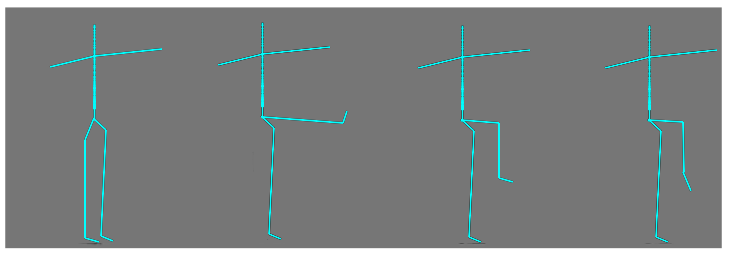
\includegraphics[width=0.6\textwidth]{forward_kinematics_skeleton.png}
    \caption{\small{Последовательное применение преобразований, начиная от копчика (корневой кости) и заканчивая ступней.}}
    %\label{fig:awesome_image}
\end{figure}


\paragraph{Применение скелета к модели}

После того как рассчитанны матрицы поворотов для скелета, их необходимо применить на вершины модели.
Для этого используется рекурсивный алгоритм похожий на алгоритм для анимации скелета. Ниже приведен его псевдокод:

\begin{small}
\begin{verbatim}
deform_mesh (bone root, mesh original, mesh deformed)
  for each child_bone of root
    for each vertex in the original mesh
      if bone_weight > 0
          apply bone global transform to vertex
          scale the resulting point by the bone weight
          store the result in deformed
      end if
    end for
    if child_bone has children
      deform_mesh (children of this node, mesh original, deformed)
    end if
  end for
end function
\end{verbatim}
\end{small}

\begin{figure}[h!]
    \centering
    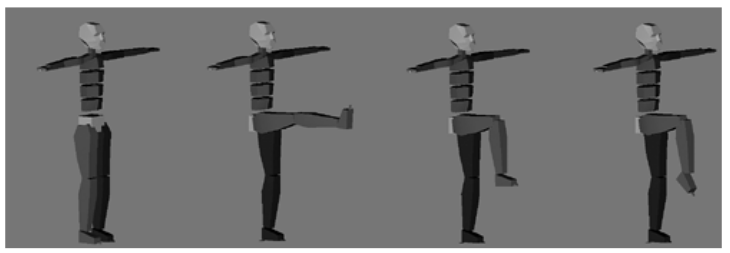
\includegraphics[width=0.8\textwidth]{forward_kinematics.png}
    \caption{\small{Применение преобразований к вершинам модели.}}

\end{figure}



\subsubsection{Реализация программы скелетной анимации}
В программе можно выделить несколько логических блоков. Каждый блок состоит из одного или более классов предоставлающих определенный функционал.

\begin{my_enumerate}
\item Блок чтения данных.
\item Блок хранения состояния анимации.
\item Блок хранения данных модели и скелета.
\item Блок деформации скелета.
\item Блок отрисовки модели.
\item Блок управления компонентами.
\end{my_enumerate}

\paragraph{Чтение данных}
С помощью библиотеки Assimp производится чтение из файла. Для оптимальной работы данные перераспределяются из структур Assimp в свои. Другие функции этой библиотеки не используются.
Ниже приведен упрощенный код считывающий информацию из файла и строящий стуктуры данных.

\begin{verbatim}
// функция для загрузки данных из библиотеки Assimp, в созданные структуры данных
public void LoadScene(byte[] filedata)
{
    using (MemoryStream fs = new MemoryStream(filedata))
    {
        _cur_scene = new SceneWrapper(ReadAssimpScene(fs, "dae"));
        // во входных данных всегда только один трек анимации
        _animation_track = _cur_scene.Animations[0];
        // примененает описания из трека анимации к скелету
        _action = new Animator(_animation_track);
        // корневая кость скелета
        BoneNode bones = _cur_scene.BuildBoneNodes("Armature");
        // модель
        Node mesh = _cur_scene.FindNode("Mesh");
        // хранит состояние анимации
        ActionState state = new ActionState();
        // объединет компоненты
        _enttity = new Entity(_cur_scene, mesh, bones, state);
    }
}
\end{verbatim}


\paragraph{Хранение состояния анимации}
Класс ActionState хранит состояние анимации. Наиболее важные поля:
\begin{itemize}
\item Трек анимации.
\item Настоящий момент времени в секундах.
\item Массив времени для всех ключевых кадров.
\end{itemize}

Фyнкция SetTime(\dots) используется для перехода к определенному моменту времени. Она находит интервал между ключевыми кадрами, подсчитывает величину интерполяции.

\begin{verbatim}
// функция для прыжка к определенному времени
public void SetTime(double time_seconds)
{            
    double time_ticks = time_seconds * TickPerSec;
    // когда время в секундах переполняеться, запускаем анимацию с начала
    double time = time_ticks % TotalDurationTicks;
    // поиск интервала между ключевыми кадрами
    int start_frame = FindStartFrameAtTime(time_seconds);
    int end_frame = (start_frame + 1) % KeyframeCount;
    // нахождение значения для интерполяции между ключевыми кадрами
    double delta_ticks = KeyframeTimes[end_frame] - KeyframeTimes[start_frame];
    // если необходимо запустить анимацию заново
    if (delta_ticks < 0.0)
    {
        delta_ticks += TotalDurationTicks;
    }
    double blend = (time - KeyframeTimes[start_frame]) / delta_ticks;
    // приписываем результаты расчетов
    OriginKeyframe = start_frame;
    TargetKeyframe = end_frame;
    KfBlend = blend;
}
\end{verbatim}


\paragraph{Хранение данных модели и скелета}
Работает со скелетом и моделью.
Реализует функции поиска костей в скелете или подмоделей в модели.
Функция BuildBones строит скелет по данным из модели (скелет как отдельный класс не существует, он определяеться корневой костью).

Ниже приведен класс описывающий кость скелета:
\begin{verbatim}
class BoneNode
{
    public string Name;
    public Matrix4 GlobalTransform;
    public Matrix4 LocalTransform;

    public BoneNode Parent;
    public List<BoneNode> Children;
    public BoneNode(Node assimp_node) { ... }
}
\end{verbatim}


\paragraph{Деформация скелета}
Применяет данные, описывающие (в матрицах поворота) новую позицию для каждой кости к костям из скелета.
То есть деформирует скелет в соответствии с моментом времени в анимации. На вход блока подается класс ActionState, содержащий информацию о состоянии анимации и корневая кость скелета.

\begin{verbatim}
// функция для извлечения матриц поворота из трека и применения их к скелету
public void ChangeLocalFixedDataBlend(ActionState st)
{
    // для каждой кости создает свой канал анимации    
    foreach (NodeAnimationChannel channel in _action.NodeAnimationChannels)
    {
        BoneNode bone_nd = _scene.GetBoneNode(channel.NodeName);
        // поворот кости
        Quaternion target_roto = Quaternion.Identity;
        if (channel.RotationKeyCount > st.TargetKeyframe)
        {
            target_roto = channel.RotationKeys[st.TargetKeyframe].Value.eToOpenTK();
        }
        Quaternion start_frame_roto = channel.RotationKeys[st.OriginKeyframe].Value;
        // интерполяция поворота между двумя ключевыми кадрами
        Quaternion result_roto = Quaternion.Slerp(start_frame_roto, target_roto, (float)st.KfBlend);
        // сдвиг кости
        Vector3 target_trans = Vector3.Zero;
        if (channel.PositionKeyCount > st.TargetKeyframe)
        {
            target_trans = channel.PositionKeys[st.TargetKeyframe].Value;
        }
        Vector3 cur_trans = channel.PositionKeys[st.OriginKeyframe].Value;
        // интерполяция сдвига между двумя ключевыми кадрами
        Vector3 result_trans = cur_trans + Vector3.Multiply(target_trans - cur_trans, (float)st.KfBlend);
        // объединение поворота и сдвига
        Matrix4 result = Matrix4.CreateFromQuaternion(result_roto);
        result.Row3.Xyz = result_trans;
        bone_nd.LocalTransform = result;
    }
}

// функция для расчета глобальной матрицы поворота для каждой кости
// эта матрица будет позднее применена к вершинам модели
private void ReCalculateGlobalTransform(BoneNode nd)
{
    nd.GlobalTransform = nd.LocalTransform * nd.Parent.GlobalTransform;
    foreach (var child in nd.Children)
    {
        ReCalculateGlobalTransform(child);
    }
}
\end{verbatim}



\paragraph{Отрисовка модели}
Загружает данные о модели в OpenGL.
Запрашивает OpenGL об отводе буферов памяти под вершины, нормали, цвета вершин и массив индексов. Применяет свойства материала, например: цвет, коэффициент рассеивания света, коэффициент свечения и т.д.

Данные o вершинах, материалах и нормалях необходимо загружать в буферы памяти расположенные на видеокарте для того что бы обеспечить приложению приемлимую скорость отрисовки.
Ниже приведен код для загрузки данных в память видеокарты:

\begin{verbatim}
// объект содержащий идентификационные номера буферов в OpenGL
struct Vbo
{
    public int VertexBufferId;
    public int NormalBufferId;
    public int ElementBufferId;
    public int NumIndices;
}

// функция для создания нового буфера 
// и заполнения его данными из массива векторов
private void NewOpenGLBufferWithFloats(out int outGlBufferId, List<Vector3D> dataBuffer) 
{
    GL.GenBuffers(1, out outGlBufferId);
    GL.BindBuffer(BufferTarget.ArrayBuffer, outGlBufferId);
    int sizeof_vec3d = 12; // X,Y,Z = 3 floats, 4 bytes each
    var byteCount = dataBuffer.Count * sizeof_vec3d;
    var temp = new float[byteCount];
    var n = 0;
    foreach(var v in dataBuffer)
    {
        temp[n++] = v.X;
        temp[n++] = v.Y;
        temp[n++] = v.Z;
    }
    GL.BufferData(BufferTarget.ArrayBuffer, (IntPtr)byteCount, temp, BufferUsageHint.StreamDraw);
    VerifyArrayBufferSize(byteCount);
    GL.BindBuffer(BufferTarget.ArrayBuffer, 0);
}

// функция для загрузки данных о модели в память видеокарты
private void Upload(out Vbo vboToFill)
{
    vboToFill = new Vbo();    
    NewOpenGLBufferWithFloats(out vboToFill.VertexBufferId, _mesh.Vertices);
    if (_mesh.HasNormals)
    {
        NewOpenGLBufferWithFloats(out vboToFill.NormalBufferId, _mesh.Normals);
    }
}

\end{verbatim}

Для создания эффекта движения нeобходимо каждый кадр менять содержимое буферов расположыенных на видеокарте.
А именно необходимо менять координаты вершин и направления нормалей к каждой вершине (для корректного отображения света/тени).
Для этого необходимо послать запрос к драйверу OpenGL и получить указатель на память с загруженными ранее данными.
Далее приведен код модифицирущий данные в буфере для следующего кадра.

\begin{verbatim}
// функция для получения доступа к буферу OpenGL
public void BeginModifyNormalData(out IntPtr data, out int qty_normals)
{
    GL.BindBuffer(BufferTarget.ArrayBuffer, _vbo.NormalBufferId);
    data = GL.MapBuffer(BufferTarget.ArrayBuffer, BufferAccess.ReadWrite);
    qty_normals = _mesh.Normals.Count;
}
// функция для освобождения буфера OpenGL
public void EndModifyNormalData()
{
    bool data_upload_ok = GL.UnmapBuffer(BufferTarget.ArrayBuffer);
    if (! data_upload_ok)
    {
        throw new Exception("OpenGL driver has failed.");
    }
}
\end{verbatim}


\paragraph{Управление компонентами}
Класс Entity объединяет компоненты необходимые для анимации одного персонажа. Хранит ссылки на скелет (корневую кость), состояние анимации (ActionState), на саму модель и на класс отрисовки модели (MeshDraw).
    \medskip
    В частности блок персонажа применяет трансформации из скелета к вершинам модели (взвешивая действие каждой кости на вершину) и модифицирует данные в буфере данных OpenGL, что и создает эффект анимации.
    
\begin{verbatim}
// функция в блоке управления компонентами для применения матриц костей к вершинам модели
public void RecursiveTransformVertices(Node node)
{
    foreach (int mesh in nd.Meshes)
    {
        // получаем указатель на буфер в OpenGL
        IntPtr pbuf_opengl;
        int qty_vertices;
        mesh.BeginModifyVertexData(out pbuf_opengl, out qty_vertices);
        // изначальная модель без деформаций
        Mesh original_data = mesh.OriginalData;
        // go over every vertex in the mesh
        unsafe
        {
            int sz = 3;         // размер шага
            float* coords = (float*)pbuf_opengl;
            for (int vertex_id = 0; vertex_id < qty_vertices; vertex_id++)
            {
                Matrix4 matrix_with_offset = mesh._vertex_id2matrix[vertex_id];
                // получить изначальные координаты вершины
                Vector3 vertex_default = original_data.Vertices[vertex_id];
                Vector3 vertex;
                Vector3.Transform(ref vertex_default, ref matrix_with_offset, out vertex);
                // Применение веса к вершине
                Vector3 delta = vertex_default - vertex;
                vertex += delta *  mesh._vertex_id2bone_weight[vertex_id];
                // Запись новых координат обратно в буфер OpenGL
                coords[vertex_id*sz + 0] = vertex.X;
                coords[vertex_id*sz + 1] = vertex.Y;
                coords[vertex_id*sz + 2] = vertex.Z;
            }
        }
        mesh.EndModifyVertexData();

        foreach (Node child in nd.Children)
        {
            RecursiveTransformVertices(child);
        }
    }
}
\end{verbatim}


\subsection{Mетод организации входных и выходных данных}

\subsubsection{Описание метода входных и выходных данных}
Входными данными является файл в формате collada (.dae)
, в котором в обязательном порядке должны присутствовать следующие элементы:
\begin{my_enumerate}
\item Одна полигональная модель.
\item Один трек анимации.
\item Один скелет.
\end{my_enumerate}

Если не выполненны условия на наличие полигональной модели,
трека анимации и связанного с моделью скелета то
у программы не хватит информации для воспроизведения анимации.

Выходными данными является отображение анимации на экране.


\subsection{Выбор состава технических средств}

\subsubsection{Состав технических и програмных средств}
Для возможности запустить приложение необходимо учесть следующие системные требования:
\begin{my_enumerate}
\item Компьютер, оснащенный:
    \begin{my_enumerate}
    \item Обязательно 64-разрядный (x64) процессор с тактовой частотой 1 гигагерц (ГГц) или выше;
    \item 512 мегабайт (ГБ) оперативной памяти (ОЗУ);
    \item 2 ГБ (для 64-разрядной системы) пространства на жестком диске;
    \item графическое устройство OpenGL с драйвером версии 3.1 или выше.
    \end{my_enumerate}
\item Монитор
\item Видеокарта
\item Мышь
\item Клавиатура
\end{my_enumerate}

\bigskip

Также необходимо учесть следующие програмные требования:
\begin{my_enumerate}
\item Поддержка OpenGL версии 3.1
\item 64-битная операционная система Windows 7.
\item .NET Framework версии 4.5.1
\item Библиотека Assimp версии 3.1
\item Библиотека OpenTK версии 1.1.4
\end{my_enumerate}

Программа была протестирована и отлажена на версии OS Windows 7 с использованием .Net Framework 4.5.1, OpenTK версии 1.1.4 и Assimp версии 3.1.

Качество и корректность работы программы при других версиях библиотек и операционных систем не проверялось.

Программа использует буферы графической памяти типа STREAM\_WRITE и функции glMapData и glSubBufferData которые в OpenGL официально поддерживаются лишь с версии 3.1

Технические требования к памяти и периферии не превышают технических требований к операционной системе Windows 7 с установленным на ней .Net Framework 4.5.1


\newpage
\section{Технико-экономические показатели}
\subsection{Ориентировачная экономическая эффективность и годовая потребность}
Ориентировочная экономическая эффективность не рассчитывается, предполагается, что программа будет использоваться пользователем несколько раз в неделю, на протяжении коротких периодов времени, т. е. количество сеансов на одном рабочем месте в год составит примерно 48 сеансов.

\subsection{Экономические преимущества разработки}
Экономические преимущества разработки в сравнении с лучшими отечественными и зарубежными аналогами рассчитаны на январь 2016 года. Существующими аналогами данного приложения являются пакеты для 3-х мерного моделлирования и анимации. В силу того что данное приложение распростроняется бесплатно, единственным экономически выгодным аналогом к нему будет программа Blender. Однако Blender гораздо более сложен в использовании и потребляет намного больше системных ресурсов (жесткой памяти, ОЗУ, времени процессора).

\newpage
\section{Источники, используемые при разработке}
\subsection{Список используемой литературы}
\begin{my_enumerate}
\item
OpenGL Superbible: Comprehensive Tutorial and Reference (7th Edition)
Graham Sellers (Author), Richard S Wright Jr. (Author), Nicholas Haemel (Author)
ISBN-13: 978-0672337475

\item
Порев В.Н. Компьютерная графика. – СПб.: БХВ-Петербург, 2002. – 432 с.: ил.

\item
ГОСТ 19.102-77 Стадии разработки. //Единая система программной документации. -М.: ИПК Издательство стандартов, 2001.

\item
ГОСТ 19.201-78 Техническое задание. Требования к содержанию и оформлению // Единая система программной документации. -М.:ИПК Издательство стандартов, 2001.

\item
ГОСТ 19.101-77 Виды программ и программных документов
//Единая система программной документации. -М.: ИПК Издательство стандартов, 2.: 001.

\item
ГОСТ 19.103-77 Обозначения программ и программных документов. //Единая система программной документации. -М.: ИПК Издательство стандартов, 2001.

\item
ГОСТ 19.104-78 Основные надписи //Единая система программной документации. -М.: ИПК Издательство стандартов, 2001.

\item 
ГОСТ 19.105-78 Общие требования к программным документам. //Единая система
программной документации. – М.: ИПК Издательство стандартов, 2001.

\end{my_enumerate}



\newpage
\section{Приложение 1. Терминология}
\subsection{Терминология}
\begin{description}

\item[Корневая вершина (англ. root node)]  
Самый верхний узел дерева.

\item[Полигональная сетка (жарг. меш от англ. polygon mesh)]
Совокупность вершин, рёбер и граней, которые определяют форму многогранного объекта в трехмерной компьютерной графике и объёмном моделировании. Гранями являются треугольники.

\item[Дерево]
Связный ациклический граф. Связность означает наличие путей между любой парой вершин, ацикличность — отсутствие циклов и то, что между парами вершин имеется только по одному пути.

\item[Степень вершины]
Количество инцидентных ей (входящих/исходящих из нее) ребер.

\item[Интерполяция, интерполирование анимации]
Способ нахождения промежуточных значений состояния анимации по имеющемуся дискретному набору известных значений.

\item[Z-буферизация]
В компьютерной трёхмерной графике способ учёта удалённости элемента изображения. Представляет собой один из вариантов решения «проблемы видимости»

\item[Z-конфликт (англ. Z–fighting)]
Если два объекта имеют близкую Z-координату, иногда, в зависимости от точки обзора, показывается то один, то другой, то оба полосатым узором.

\item[OpenGL (Open Graphics Library)]
Спецификация, определяющая независимый от языка программирования платформонезависимый программный интерфейс для написания приложений, использующих двумерную и трёхмерную компьютерную графику. На платформе Windows конкурирует с Direct3D.

\item[Рендеринг (англ. rendering — «визуализация»)]
Термин в компьютерной графике, обозначающий процесс получения изображения по модели с помощью компьютерной программы.

\item[Текстура]
Растровое изображение, накладываемое на поверхность полигональной модели для придания ей цвета, окраски или иллюзии рельефа. Приблизительно использование текстур можно легко представить как рисунок на поверхности скульптурного изображения.

\end{description}



\newpage
\section{Приложение 2. Формат Collada (.dae)}
Collada — это формат, разработанный для обмена  информацией между 3D приложениями.
Управляется некоммерческой организацией Khronos Group. Collada использует открытый стандарт XML для обмена форматами, которые в противном случае были бы несовместимы. Collada был задуман как промежуточный формат для переноса файлов.
Реализована поддержка в таких программах, как Maya, 3ds Max, Blender.
Ниже приведен пример описания квадрата в формате collada:
\begin{small}
\begin{verbatim}
<?xml version="1.0" encoding="utf-8"?>
<COLLADA xmlns="http://www.collada.org/2005/11/COLLADASchema" version="1.4.1">
  <asset>
    <unit name="meter" meter="1"/>
    <up_axis>X_UP</up_axis>
  </asset>
  <library_images/>
  <library_geometries>
    <geometry id="Plane_001-mesh" name="Plane.001">
      <mesh>
        <source id="Plane_001-mesh-positions">
          <float_array id="Plane_001-mesh-positions-array" count="12">-1 -1 0 1 -1 0 -1 1 0 1 1 0</float_array>
          <technique_common>
            <accessor source="#Plane_001-mesh-positions-array" count="4" stride="3">
              <param name="X" type="float"/>
              <param name="Y" type="float"/>
              <param name="Z" type="float"/>
            </accessor>
          </technique_common>
        </source>
        <source id="Plane_001-mesh-normals">
          <float_array id="Plane_001-mesh-normals-array" count="3">0 0 1</float_array>
          <technique_common>
            <accessor source="#Plane_001-mesh-normals-array" count="1" stride="3">
              <param name="X" type="float"/>
              <param name="Y" type="float"/>
              <param name="Z" type="float"/>
            </accessor>
          </technique_common>
        </source>
        <polylist count="2">
          <input semantic="VERTEX" source="#Plane_001-mesh-vertices" offset="0"/>
          <input semantic="NORMAL" source="#Plane_001-mesh-normals" offset="1"/>
          <vcount>3 3 </vcount>
          <p>1 0 3 0 2 0 0 0 1 0 2 0</p>
        </polylist>
      </mesh>
    </geometry>
  </library_geometries>
  <library_visual_scenes>
    <visual_scene id="Scene" name="Scene">
      <node id="Plane_001" name="Plane_001" type="NODE">
        <matrix sid="transform">69.99999 0 0 0 0 5.28485e-6 -69.99999 0 0 69.99999 5.28485e-6 0 0 0 0 1</matrix>
        <instance_geometry url="#Plane_001-mesh" name="Plane_001"/>
      </node>
    </visual_scene>
  </library_visual_scenes>
  <scene>
    <instance_visual_scene url="#Scene"/>
  </scene>
</COLLADA>
\end{verbatim}
\end{small}

\newpage
\section{Приложение 3. Описание классов}

\subsection{Класс Action\+State}
\label{class_win_form_animation2_d_1_1_action_state}\index{Action\+State@{Action\+State}}


Базовые классы\+:Base\+For\+Event\+Driven.



\subsubsection{Подробное описание}
This class knows what argumets to pass to Node\+Interpolator 


\subsection{Класс Camera\+Device}
\label{class_win_form_animation2_d_1_1_camera_device}\index{Camera\+Device@{Camera\+Device}}


Maintains camera abstraction. Allows support for orbiting, free fly and even 2D camera.  


\subsubsection*{Открытые члены}
\begin{DoxyCompactItemize}
\item 
{\bf Camera\+Device} (Matrix4 opengl\+\_\+init\+\_\+mat)\label{class_win_form_animation2_d_1_1_camera_device_a59ce26ab0cd14b001e61b428cbbd3993}

\begin{DoxyCompactList}\small\item\em Constructor. \end{DoxyCompactList}\item 
Vector3 {\bf Convert\+Screen2\+World\+Coordinates} (Point screen\+\_\+coords)\label{class_win_form_animation2_d_1_1_camera_device_ac7ad419940551e2a63d36549481ff424}

\begin{DoxyCompactList}\small\item\em Get the mouse position and calculate the world coordinates based on the screen coordinates. \end{DoxyCompactList}\item 
Matrix4 {\bf Matrix\+To\+Open\+GL} ()\label{class_win_form_animation2_d_1_1_camera_device_a708b9cba847463c03fc39aa0e6a8e51b}

\begin{DoxyCompactList}\small\item\em Get the camera matrix to be uploaded to drawing 2D. \end{DoxyCompactList}\item 
void {\bf On\+Mouse\+Move} (int x, int y)\label{class_win_form_animation2_d_1_1_camera_device_a91b06ea84daf2da1d561b318a0b030e3}

\begin{DoxyCompactList}\small\item\em Respond to mouse events. \end{DoxyCompactList}\item 
void {\bf Scroll} (float scroll)\label{class_win_form_animation2_d_1_1_camera_device_ab68f5c2e2b82440495f6735ec5b4a389}

\begin{DoxyCompactList}\small\item\em Zoom in/out of the scene. \end{DoxyCompactList}\end{DoxyCompactItemize}
\subsubsection*{Свойства}
\begin{DoxyCompactItemize}
\item 
Cam\+Mode {\bf \+\_\+cam\+\_\+mode}\hspace{0.3cm}{\ttfamily  [get]}\label{class_win_form_animation2_d_1_1_camera_device_a162958083b16cbc267e6f23c7392e2a5}

\begin{DoxyCompactList}\small\item\em Return the currently active camera mode. \end{DoxyCompactList}\item 
Vector3 {\bf Get\+Translation}\hspace{0.3cm}{\ttfamily  [get]}\label{class_win_form_animation2_d_1_1_camera_device_a6b52b857e583f1524e339f87102d6050}

\begin{DoxyCompactList}\small\item\em Get the translation part of the camera matrix. \end{DoxyCompactList}\end{DoxyCompactItemize}


\subsubsection{Подробное описание}
Maintains camera abstraction. Allows support for orbiting, free fly and even 2D camera. 


\subsection{Класс Draw\+Config}
\label{class_win_form_animation2_d_1_1_draw_config}\index{Draw\+Config@{Draw\+Config}}
\subsubsection*{Открытые атрибуты}
\begin{DoxyCompactItemize}
\item 
bool {\bf Enable\+Texture2D} = false
\end{DoxyCompactItemize}


\subsubsection{Подробное описание}
This class will be passed to the \doxyref{Entity}{стр.}{class_win_form_animation2_d_1_1_entity}\textquotesingle{}s Get\+Settings() so it make the scene look best. 

\subsubsection{Данные класса}
\index{Win\+Form\+Animation2\+D\+::\+Draw\+Config@{Win\+Form\+Animation2\+D\+::\+Draw\+Config}!Enable\+Texture2D@{Enable\+Texture2D}}
\index{Enable\+Texture2D@{Enable\+Texture2D}!Win\+Form\+Animation2\+D\+::\+Draw\+Config@{Win\+Form\+Animation2\+D\+::\+Draw\+Config}}
\paragraph[{Enable\+Texture2D}]{\setlength{\rightskip}{0pt plus 5cm}bool Enable\+Texture2D = false}\label{class_win_form_animation2_d_1_1_draw_config_ab0185dd3fb4ebf71f25125334556bf8f}
Open\+GL settings here is a template\+: public bool \+\_\+enable = false; 
\subsection{Класс Entity}
\label{class_win_form_animation2_d_1_1_entity}\index{Entity@{Entity}}


Represents the currently loaded object. One day we will have lots of these.  


\subsubsection*{Открытые члены}
\begin{DoxyCompactItemize}
\item 
void {\bf Recursive\+Calculate\+Vertex\+Transform} (Node nd, Matrix4x4 current)\label{class_win_form_animation2_d_1_1_entity_a4f652bc4baf5a8f594384aab653088bf}

\begin{DoxyCompactList}\small\item\em Find the appropriate matrix to apply to the given vertex. \end{DoxyCompactList}\item 
void {\bf Render\+Model} ({\bf Draw\+Config} settings)\label{class_win_form_animation2_d_1_1_entity_ae7e350876ed1f078eb5a780c03b473a4}

\begin{DoxyCompactList}\small\item\em Render the model stored in Entity\+Scene useing the \doxyref{Draw\+Config}{стр.}{class_win_form_animation2_d_1_1_draw_config} settings object. \end{DoxyCompactList}\item 
void {\bf Update\+Model} (double dt\+\_\+ms)\label{class_win_form_animation2_d_1_1_entity_a069d68a65dcb75e1b3c2cd2c3c5ca99b}

\begin{DoxyCompactList}\small\item\em Deform the model vertices to align with the skeleton. \end{DoxyCompactList}\end{DoxyCompactItemize}
\subsubsection*{Открытые статические члены}
\begin{DoxyCompactItemize}
\item 
static void {\bf Transform\+Position\+Assimp} (ref Vector3D pos, ref Matrix4x4 mat, out Vector3D result)
\begin{DoxyCompactList}\small\item\em Transform a Position by the given Matrix. Based on open\+TK compatiability vector 3 class. \end{DoxyCompactList}\end{DoxyCompactItemize}


\subsubsection{Подробное описание}
Represents the currently loaded object. One day we will have lots of these. 



\subsubsection{Методы}
\index{Win\+Form\+Animation2\+D\+::\+Entity@{Win\+Form\+Animation2\+D\+::\+Entity}!Transform\+Position\+Assimp@{Transform\+Position\+Assimp}}
\index{Transform\+Position\+Assimp@{Transform\+Position\+Assimp}!Win\+Form\+Animation2\+D\+::\+Entity@{Win\+Form\+Animation2\+D\+::\+Entity}}
\paragraph[{Transform\+Position\+Assimp(ref Vector3\+D pos, ref Matrix4x4 mat, out Vector3\+D result)}]{\setlength{\rightskip}{0pt plus 5cm}static void Transform\+Position\+Assimp (
\begin{DoxyParamCaption}
\item[{ref Vector3D}]{pos, }
\item[{ref Matrix4x4}]{mat, }
\item[{out Vector3D}]{result}
\end{DoxyParamCaption}
)\hspace{0.3cm}{\ttfamily [static]}}\label{class_win_form_animation2_d_1_1_entity_a33a723df0a875e102291644e659de2b1}


Transform a Position by the given Matrix. Based on open\+TK compatiability vector 3 class. 


\begin{DoxyParams}{Аргументы}
{\em pos} & The position to transform\\
\hline
{\em mat} & The desired transformation\\
\hline
{\em result} & The transformed position\\
\hline
\end{DoxyParams}

\subsection{Класс Geometry}
\label{class_win_form_animation2_d_1_1_geometry}\index{Geometry@{Geometry}}
\subsubsection*{Открытые члены}
\begin{DoxyCompactItemize}
\item 
{\bf Geometry} (I\+List$<$ Mesh $>$ scene\+\_\+meshes, Node nd, Bone\+Node armature)\label{class_win_form_animation2_d_1_1_geometry_abd05402398b233a02784515ecd0d329e}

\end{DoxyCompactItemize}


\subsubsection{Подробное описание}
Stores info on extra geometry of the entity. 
\subsection{Класс Mesh\+Draw}
\label{class_win_form_animation2_d_1_1_mesh_draw}\index{Mesh\+Draw@{Mesh\+Draw}}
\subsubsection*{Открытые члены}
\begin{DoxyCompactItemize}
\item 
{\bf Mesh\+Draw} (Mesh mesh, I\+List$<$ Material $>$ materials)
\item 
void {\bf Render\+V\+BO} ()
\end{DoxyCompactItemize}


\subsubsection{Подробное описание}
Mesh rendering using V\+B\+Os. 

Based on {\tt http\+://www.\+opentk.\+com/files/\+T08\+\_\+\+V\+B\+O.\+cs} 

\subsubsection{Конструктор(ы)}
\index{Win\+Form\+Animation2\+D\+::\+Mesh\+Draw@{Win\+Form\+Animation2\+D\+::\+Mesh\+Draw}!Mesh\+Draw@{Mesh\+Draw}}
\index{Mesh\+Draw@{Mesh\+Draw}!Win\+Form\+Animation2\+D\+::\+Mesh\+Draw@{Win\+Form\+Animation2\+D\+::\+Mesh\+Draw}}
\paragraph[{Mesh\+Draw(\+Mesh mesh, I\+List$<$ Material $>$ materials)}]{\setlength{\rightskip}{0pt plus 5cm}{\bf Mesh\+Draw} (
\begin{DoxyParamCaption}
\item[{Mesh}]{mesh, }
\item[{I\+List$<$ Material $>$}]{materials}
\end{DoxyParamCaption}
)}\label{class_win_form_animation2_d_1_1_mesh_draw_a70daeba67e8888df740583158e434490}


Uploads the data to the G\+PU. 



\subsubsection{Методы}
\index{Win\+Form\+Animation2\+D\+::\+Mesh\+Draw@{Win\+Form\+Animation2\+D\+::\+Mesh\+Draw}!Render\+V\+BO@{Render\+V\+BO}}
\index{Render\+V\+BO@{Render\+V\+BO}!Win\+Form\+Animation2\+D\+::\+Mesh\+Draw@{Win\+Form\+Animation2\+D\+::\+Mesh\+Draw}}
\paragraph[{Render\+V\+B\+O()}]{\setlength{\rightskip}{0pt plus 5cm}void Render\+V\+BO (
\begin{DoxyParamCaption}
{}
\end{DoxyParamCaption}
)}\label{class_win_form_animation2_d_1_1_mesh_draw_a7735f3e5b99af7ffb9e8343a36c3d688}


Render mesh from G\+PU memory. The pipeline is restored afterwards. 


\subsection{Класс Mouse\+State}
\label{class_win_form_animation2_d_1_1_mouse_state}\index{Mouse\+State@{Mouse\+State}}
\subsubsection*{Открытые члены}
\begin{DoxyCompactItemize}
\item 
void {\bf Record\+Mouse\+Click} (Mouse\+Event\+Args e)\label{class_win_form_animation2_d_1_1_mouse_state_a90501009d4cbf911a31d880523548f63}

\item 
void {\bf Record\+Mouse\+Move} (Mouse\+Event\+Args e)\label{class_win_form_animation2_d_1_1_mouse_state_afa4a1b4f3fc39ff61fd13d7ba3e5d628}

\end{DoxyCompactItemize}
\subsubsection*{Открытые атрибуты}
\begin{DoxyCompactItemize}
\item 
Point {\bf Click\+Pos}\label{class_win_form_animation2_d_1_1_mouse_state_aff1227a0577100876a98c04ad407d9f4}

\item 
Point {\bf Current\+Pos}\label{class_win_form_animation2_d_1_1_mouse_state_aa03fd24e8bc7ea3e7ed22a9c564cb650}

\item 
readonly int {\bf Horiz\+Hysteresis} = 4\label{class_win_form_animation2_d_1_1_mouse_state_a2564dfd90e7599c1f850ecc35b4243ea}

\item 
Open\+T\+K.\+Vector3 {\bf Inner\+World\+Click\+Pos}\label{class_win_form_animation2_d_1_1_mouse_state_a2ba32d9d742f09b887d7487ead69490c}

\item 
Open\+T\+K.\+Vector3 {\bf Inner\+World\+Pos}\label{class_win_form_animation2_d_1_1_mouse_state_ae4a531cfd584f7535a84d3491c0d233a}

\end{DoxyCompactItemize}


\subsubsection{Подробное описание}
Simple class to store mouse status data. Monitor mouse status (delta, position, click\+\_\+position, etc.) 


\subsection{Класс Renderer}
\label{class_win_form_animation2_d_1_1_renderer}\index{Renderer@{Renderer}}


Class to control open\+GL settings and do the actual drawing. All open\+GL calls will be here.  


\subsubsection*{Открытые члены}
\begin{DoxyCompactItemize}
\item 
void {\bf Clear\+Opengl\+Frame\+For\+Render} (Matrix4 camera\+\_\+matrix)\label{class_win_form_animation2_d_1_1_renderer_acd8d4d779a35f8f11a38b158c525cae5}

\begin{DoxyCompactList}\small\item\em Prepare to render next Open\+GL frame. Clear depth/color buffers. \end{DoxyCompactList}\item 
void {\bf Draw\+Axis3D} ()
\begin{DoxyCompactList}\small\item\em Important points to remember\+: Set normals. Must be clock wise vertex draw order The x-\/axis is accross the screen, so the Z-\/axis triangle must have component along X\+: +-\/1 since look at looks towards the center, we need to offset it a bit to see the Z axis. \end{DoxyCompactList}\item 
void {\bf Init\+Open\+GL} ()\label{class_win_form_animation2_d_1_1_renderer_a8690e89b528f55a820f4e52ab09e43c7}

\begin{DoxyCompactList}\small\item\em Enable default Open\+GL settings. Set lights, material, etc. Call this once in the beginning. \end{DoxyCompactList}\item 
void {\bf Resize\+Open\+GL} (int width, int height)\label{class_win_form_animation2_d_1_1_renderer_aeeebebac1bb2809f36e94795d29c706c}

\begin{DoxyCompactList}\small\item\em Called when window size changes. \end{DoxyCompactList}\end{DoxyCompactItemize}


\subsubsection{Подробное описание}
Class to control open\+GL settings and do the actual drawing. All open\+GL calls will be here. 



\subsubsection{Методы}
\index{Win\+Form\+Animation2\+D\+::\+Renderer@{Win\+Form\+Animation2\+D\+::\+Renderer}!Draw\+Axis3D@{Draw\+Axis3D}}
\index{Draw\+Axis3D@{Draw\+Axis3D}!Win\+Form\+Animation2\+D\+::\+Renderer@{Win\+Form\+Animation2\+D\+::\+Renderer}}
\paragraph[{Draw\+Axis3\+D()}]{\setlength{\rightskip}{0pt plus 5cm}void Draw\+Axis3D (
\begin{DoxyParamCaption}
{}
\end{DoxyParamCaption}
)}\label{class_win_form_animation2_d_1_1_renderer_a78178415342aec84aff33ff22fd711eb}


Important points to remember\+: Set normals. Must be clock wise vertex draw order The x-\/axis is accross the screen, so the Z-\/axis triangle must have component along X\+: +-\/1 since look at looks towards the center, we need to offset it a bit to see the Z axis. 


\subsection{Интерфейс I\+Transform\+State}
\label{interface_win_form_animation2_d_1_1_i_transform_state}\index{I\+Transform\+State@{I\+Transform\+State}}


Implement this when class allows local matrix transforms. (\doxyref{Entity}{стр.}{class_win_form_animation2_d_1_1_entity}, Camera)  




Производные классы\+:Camera\+Drawing2D и Camera\+Free\+Fly3D.

\subsubsection*{Открытые члены}
\begin{DoxyCompactItemize}
\item 
void {\bf Move\+By} (Vector3 direction)\label{interface_win_form_animation2_d_1_1_i_transform_state_a18642041c99d4296d1c64b247293cea2}

\begin{DoxyCompactList}\small\item\em x,y,z should be direction parameters, one of \{-\/1, 0, 1\}. Called on keyboard events. \end{DoxyCompactList}\item 
void {\bf Rotate\+By} (double angle\+\_\+degrees)\label{interface_win_form_animation2_d_1_1_i_transform_state_a9d5f016db4f3ff2ad068fe06c46e812d}

\begin{DoxyCompactList}\small\item\em Rotate by angle around default axis. Called on mouse events. \end{DoxyCompactList}\end{DoxyCompactItemize}
\subsubsection*{Свойства}
\begin{DoxyCompactItemize}
\item 
Vector3 {\bf Get\+Translation}\hspace{0.3cm}{\ttfamily  [get]}\label{interface_win_form_animation2_d_1_1_i_transform_state_a6b52b857e583f1524e339f87102d6050}

\begin{DoxyCompactList}\small\item\em Get the translation part of the matrix. \end{DoxyCompactList}\end{DoxyCompactItemize}


\subsubsection{Подробное описание}
Implement this when class allows local matrix transforms. (\doxyref{Entity}{стр.}{class_win_form_animation2_d_1_1_entity}, Camera) 




% Index
\newpage

\eskdListOfChanges

% \phantomsection
% \addcontentsline{toc}{section}{Алфавитный указатель}
% \printindex

\end{document}
